\chapter{Implementation}

\section{Installing gateways in Furtwangen}

\ac{TTNM} already had a number of data points for existing \ac{LoRaWAN} gateways in the Furtwangen area.
However, to make a good geolocation prediction for a \ac{LoRaWAN} node, it is necessary to have at least three gateways in range of the node.

Since, at the beginning of this thesis, there were only two gateways installed in the vicinity of Furtwangen, the first step was to research, order and then install additional gateways in the city.

Some gateways that were used in this thesis were ones that were already in the possession of the \ac{HFU}.
Such was the case for the \emph{Dragino LG308 / LG308N} indoor gateways as well as a \emph{RAK7258} indoor gateway.

Additionally, for development purposes, a \emph{Dragino PG1301} gateway was also used.
The PG1301 is designed to be used with a Raspberry Pi and mounts on top of it in typical Raspberry Pi shield fashion.

\subsection{Researching gateways}

Two MikroTik wAP LR8 kit gateways were purchased for the thesis.
They were chosen after recommendation by a member of the \ac{HSN-TTN} team~\cite{hochschwarzwald_smart_net_-_thethingsnetwork_eingesetzte_nodate}.
The MikroTik wAP LR8 kit was a compelling offer due to its low price and the fact that it comes with MikroTik's \emph{RouterOS}, a well-established GUI for configuring networking devices~\cite{mikrotik_mikrotik_nodate}.
A picture of this gateway can be seen in \cref{pic:mikrotik-lr8-kit-gateway}.
The antenna used with the MikroTik wAP LR8 kit is also from MikroTik, which is a 6.5 dBi antenna which can be seen in \cref{pic:mikrotik-antenna-c-building}.

The other gateway that was purchased for the thesis was a \emph{Dragino DLOS8N} outdoor gateway.
This gateway was chosen because of difficulties in ordering the second MikroTik wAP LR8 kit.
It was available right away at the time of ordering and was thus chosen as a short-term replacement.
It was used even after the second LR8 arrived as the user interface is identical to the one used in the Dragino LG308 gateway which made it easy to set up.
The DLOS8N also has a case that is weatherproof and made for outdoor use, making it similarly suitable as the LR8.

\subsection{Locations}

% TODO: Add map with Gateway locations (later)

Multiple locations proved themselves to be worth considering when it came to installing new \ac{LoRaWAN} gateways in Furtwangen.
In the following sections, the chosen locations are described and evaluated.

\subsubsection{\ac{HFU} B and C building}

% TODO add more info about gateway deployments?

The first antenna and gateway installed was a Dragino LG308 connected to a MikroTik antenna on top of the \ac{HFU} C building as seen in \cref{pic:mikrotik-antenna-c-building}.
While not as high in altitude as the \ac{GHB} building, it was thought to still be a good location to receive signals from the surrounding area.
The roof of the C building is located in an exposed in the middle of the valley Furtwangen is situated in.

Another gateway with antenna was deployed on top of the B building as there already was ample infrastructure available.
A Dragino DLOS8N gateway was used here because of its ability to easily be powered by \ac{PoE}.

\subsubsection{\acf{GHB} and \acf{ASH} student dormitories}

The \ac{GHB} is a popular student dormitory located on the Großhausberg mountainside in Furtwangen.
Its exposed location and the fact that it is among the highest buildings in the city makes it a good location for putting up a \ac{LoRaWAN} gateway.

The network infrastructure of both the \ac{GHB} and the \ac{ASH} are managed by the ``\ac{GHB} netadmins'' who are students of \ac{HFU}.
With their help, it was possible to install antennas on the roofs of the \ac{GHB} and \ac{ASH} student dormitories.

\begin{figure}[h]
    \centering
    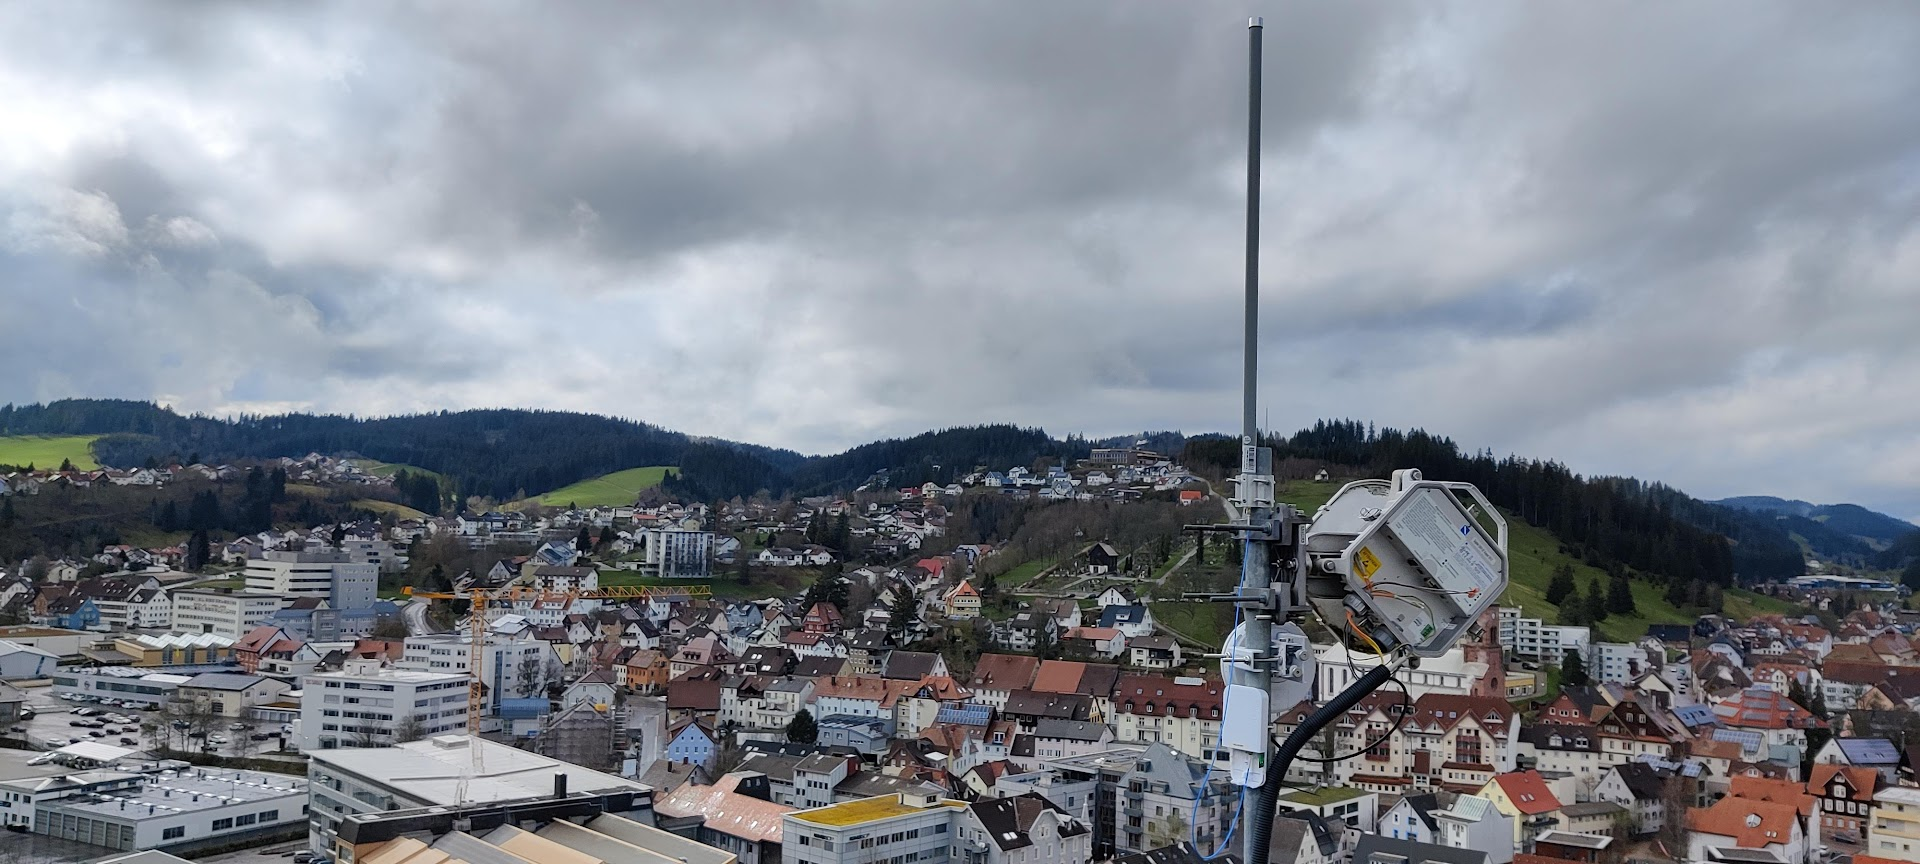
\includegraphics[width=1\textwidth]{pictures/hardware/gateway-deployment/lr8_ghb_installation.jpg}
    \caption{Installed MikroTik LR8 wAP with antenna on the GHB student dormitory\label{pic:mikrotik-gateway-ghb-installation}}
\end{figure}

\Cref{pic:mikrotik-gateway-ghb-installation} shows the installed MikroTik wAP LR8 kit gateway on the roof of the \ac{GHB} student dormitory.
Again, \ac{PoE} was used to power the gateway since only one cable needed to be put through the existing cable duct.

\section{Collecting additional \acf{TTNM} data in the Furtwangen area}

In order to have more data to work with as far as geolocation calculations are concerned, there was a need to collect more \ac{LoRaWAN}, \ac{RSSI} and \ac{GPS} data that could be synthesized.
This was done by using \ac{LoRaWAN} nodes that were equipped with \ac{GPS} modules and then moving them around the city of Furtwangen.

\subsection{Used \acs{LoRa} nodes}

In this chapter, the \ac{LoRa} nodes used for collecting \ac{GPS} data for \ac{TTNM} are described are briefly evaluated.

\subsection{ELV LW experimental platform}

\begin{figure}[h]
    \centering
    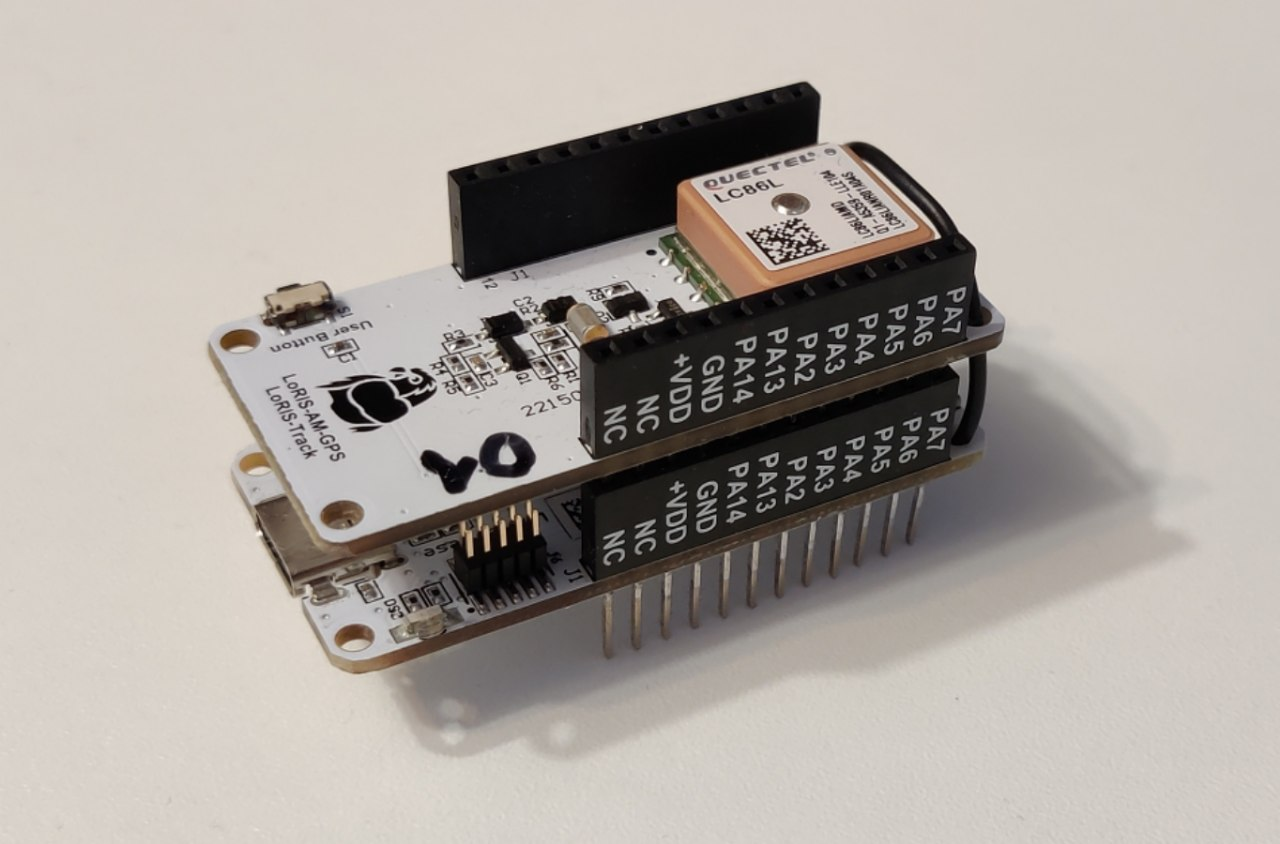
\includegraphics[width=0.5\textwidth]{pictures/hardware/gps-nodes/loris_bare.jpg}
    \caption{ELV-AM-GPS \ac{LoRaWAN} node on top of the LoRIS base\label{pic:loris-node-bare}}
\end{figure}

The ELV LW experimental platform was the \ac{LoRaWAN} node out of the ones used during this thesis that worked best out of the box as far as overall usability is concerned\cite{elv_elektronik_ag_elv-lw-base_2023}.
The ELV LW experimental platform consists of a base module called ELV-BM-TRX1 and a number of different sensor modules that can be stacked on top of it as seen in \cref{pic:loris-node-bare}.
It has a USB-C port, which made powering the tracker with an external power bank simple.

Little had to be done in order to begin using the base with the additional \ac{GPS} module ELV-AM-GPS~\cite{elv_elektronik_ag_elv-track_2022}.
Flashing the firmware using a tool provided by the manufacturer was the first step.
Additionally, the \ac{OTAA} credentials provided in the box of the base LoRIS module had to be entered into \ac{TTN}.

\begin{figure}[h]
    \centering
    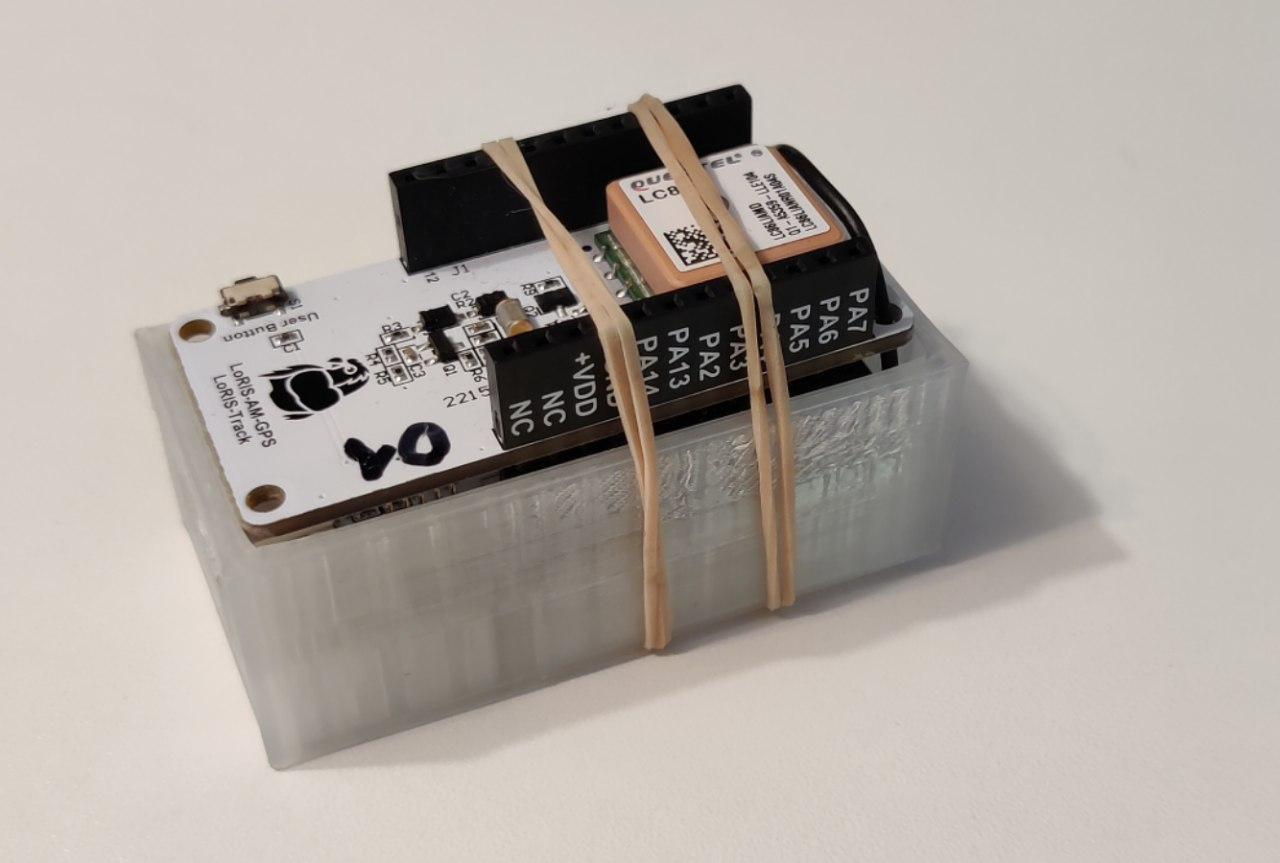
\includegraphics[width=0.5\textwidth]{pictures/hardware/gps-nodes/loris_with_case.jpg}
    \caption{ELV-AM-GPS \ac{LoRaWAN} node in self-designed 3D printed case\label{pic:loris-node-with-case}}
\end{figure}

To make the board a little more robust, a 3D printed case was designed in Fusion 360 and printed as can be seen in~\cref{pic:loris-node-with-case}.

\subsection{ELV \acs{GPS} Tracker}

\begin{figure}[h]
    \centering
    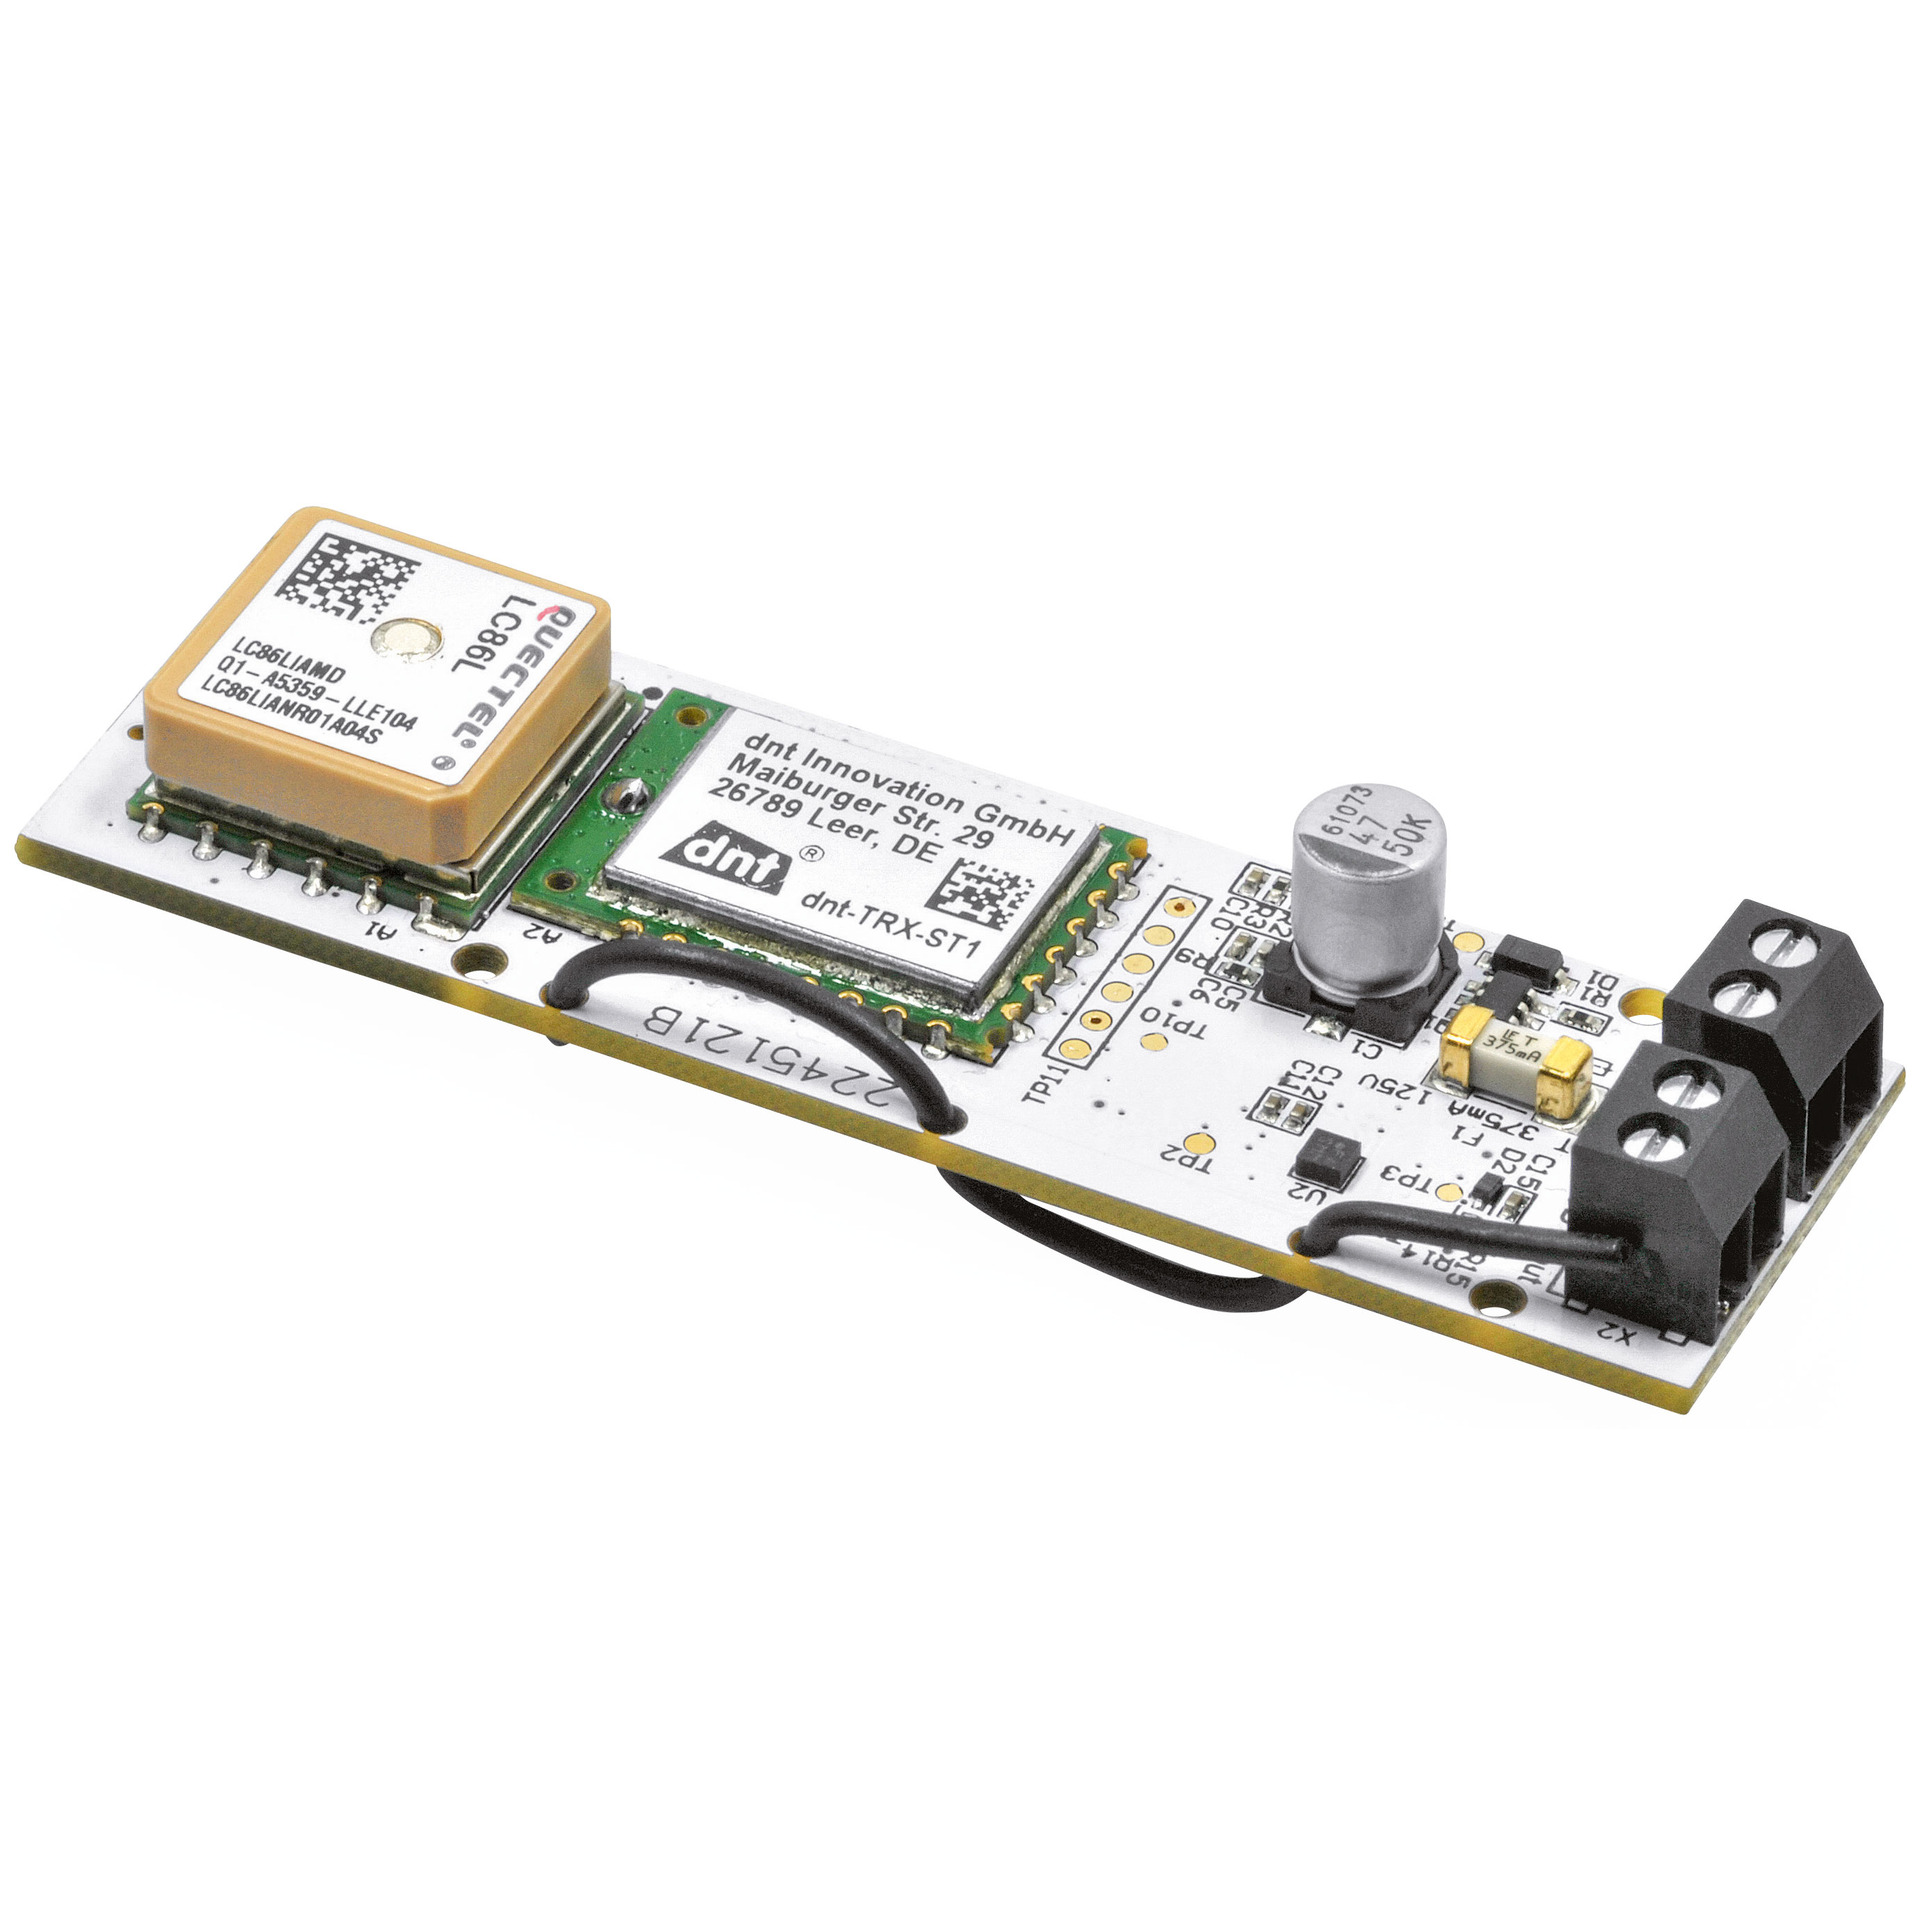
\includegraphics[width=0.6\textwidth]{pictures/hardware/gps-nodes/ELV-LW-GPS1.jpg}
    \caption{ELV-LW-GPS1 \ac{LoRaWAN} node~\protect\cite{elv_elektronik_ag_elv_2023}}
\end{figure}

The ELV-LW-GPS1 is another \ac{LoRaWAN} node that is designed to be used as a \ac{GPS} tracker.
Its specialty is that it takes a power source that can range from 5 to 40 volts.
This fact makes it flexible in terms of power supply and makes it possible to use it, for example, with a car battery that usually has a voltage of 12 volts.

Find a power source to use it for this thesis was a bit of a challenge.
It can be powered by a 9V battery.
Those, however, usually have a low capacity and are not rechargeable.

% TODO how was this solved?


\subsection{Heltec HTCC-AB02S}

% didn't work well enough without additional GPS antenna
% screen is pretty nice, though

% TODO
\subsection{dnt-LW-ATS}

\begin{figure}[h]
    \centering
    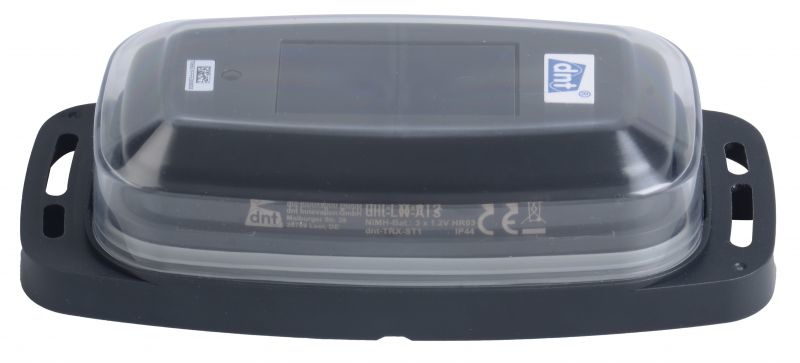
\includegraphics[width=0.6\textwidth]{pictures/hardware/gps-nodes/dnt-LW-ATS.jpg}
    \caption{dnt-LW-ATS \ac{LoRaWAN} node~\protect\cite{dnt_gmbh_dnt_nodate}}
\end{figure}

At first glance, this was the most promising \ac{LoRa} node for the task at hand.
It has a built-in \ac{GPS} module as well as a weatherproof, IP44 rated exterior case and a solar panel for charging the internal battery.

However, the node proved to be difficult to configure and use.
The device offers a \emph{motion based cyclic} mode in which, during physical movement, the node sends its \ac{GPS} coordinates to \ac{TTN} every few seconds.
This, however, did not work in practice and the node would only send its coordinates very irregularly, if at all.
The documentation was not very helpful with finding the root cause and the manufacturer also could only offer to replace the hardware.

\section{Program structure: \acf{TTNL}}\label{section:ttnl}

The programmatic implementation of this thesis was called \acf{TTNL} and split into two parts: the backend and the frontend.

\subsection{Overview}

% TODO add diagram of program structure

\subsection{Database}

% TODO add ER diagram of database

\subsection{Used technologies - Backend}

% TODO

\subsubsection{Node.js}

\subsubsection{\acf{JS} / \acf{TS}}

\subsubsection{Express}

\subsubsection{Prisma}

\subsubsection{PostgreSQL}

\subsubsection{Jest for testing}

\subsection{Used technologies - Frontend}

\subsubsection{Vue.js}

Vue.js is a \ac{JS} framework for building reactive user interfaces~\cite{evan_you_vuejs_2023}.
It was used in this thesis as a means to implement the frontend of the \ac{TTNL} web application.

\subsubsection{Vuetify}

Vuetify is a \ac{UI} framework for Vue.js that provides components that are based on Google's Material Design guidelines~\cite{vuetify_vuetify_2023}\cite{google_llc_material_nodate}.
In this thesis, Vuetify was used as a modern looking \ac{UI} framework for the frontend of the \ac{TTNL} web application.
Its usage as import-able predefined Vue components also allowed for a quick and easy implementation of the frontend.

\subsubsection{Leaflet}

\subsubsection{GeoJSON}

GeoJSON is a format used for representing geographical data using the popular \ac{JSON} format~\cite{butler_geojson_2016}.

\subsection{Locating \acs{LoRaWAN} nodes with multiple techniques}

\subsubsection{First idea: Fixed \ac{RSSI} to range scale}

% TODO add plot of fixed RSSI to range scale function to generate ranges for multilateration
\subsubsection{\ac{RSSI}-based multilateration}

\paragraph{Plotting \ac{RSSI} to range from existing data}

% TODO add positive and negative RSSI range plots as image examples and explain them

\subsubsection{\ac{ToA}-based multilateration}

% TODO describe (with some data) why this didn't work (timestamps are not accurate enough and also sometimes way off)

\subsubsection{Fingerprinting with \ac{RSSI} values}

% Show how this worked (quite alright, but needs a lot of pre-existing data)